\documentclass[11pt]{scrartcl}
\setkomafont{disposition}{\normalfont\bfseries}
\usepackage[utf8]{inputenc}
\usepackage{fullpage}
\usepackage[parfill]{parskip}
\usepackage{graphicx}
\usepackage{amsmath}






\title{Final Project Prospectus}
\subtitle{{Sentiment Analysis of Steam Review Datasets}}

\author{Junjie Lei}
\date{October 17, 2020}

\begin{document}

\maketitle

\section*{Background \&\& Objectives}
Sentiment analysis or opinion mining is one of the major topics in Natural Language Processing and Text Mining. \textbf{This final project will provide a complete process of sentiment analysis from data preparation to final classification on a user-generated sentimental dataset}.

Global video game market is a large market with more than $100$ billion dollars annually and the market is still growing rapidly. Here is the global game market predictions by \textit{Newzoo}: 

\begin{figure}[!ht]
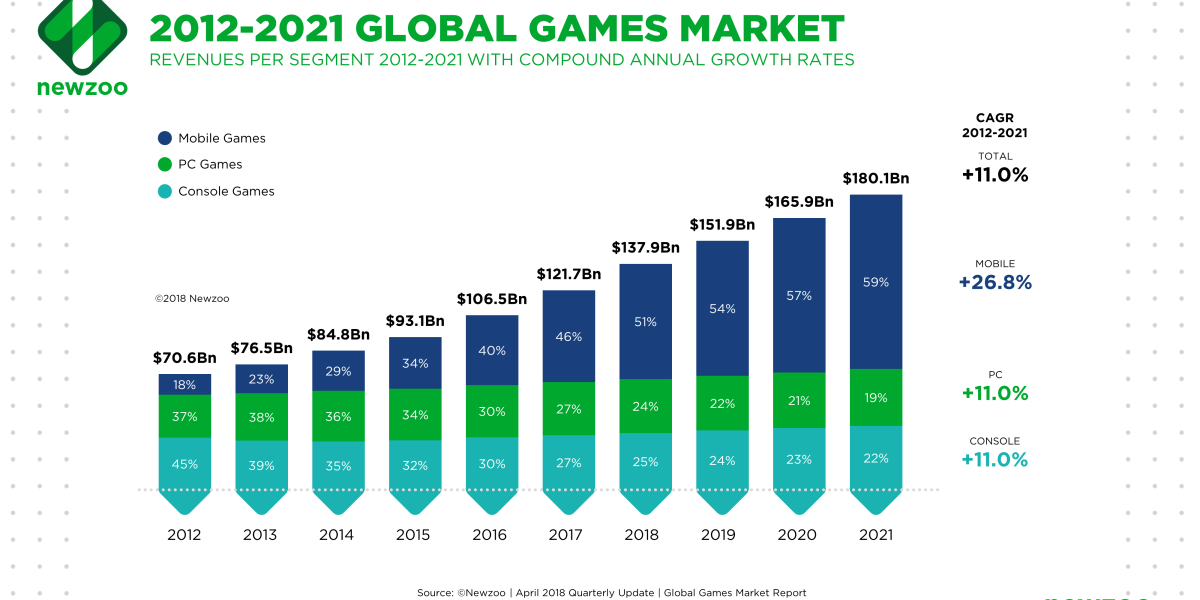
\includegraphics{prediction.png}
\centering
\end{figure}

Very unlike traditional products, digital products such as games in most of the cases can be only purchased online. Poeple normally cannot try the products before purchasing them. In addition, people are less likely to get refunds after the transactions were made. Therefore, reviews may be the only source that people can know about the products' user experience before purchasing. Sentiment analysis can be very ncecessry and useful for game products. 

According to Fang 2015, ``sentiment is an attitude or judgment based on feelings or experiences". For online stores or online market, former reviews can play an important role in customer’s decision making process, which indicates that an accurate prediction of sentiment from a certain review can increase potential profit.



\section*{Data Source}
The data used for this fianl project  is the Steam Review Dataset. Steam, developed by Valve Corporation, is one of the world largest PC game distribution platform. Its community members provide insightful information in terms of their opinion on games or other softwares. 
The main data grathering/collection methods are listed as following:

\begin{itemize}

    \item Steam Database \\ 
    Real time data has been collected and processed in several sites such as SteamDB and SteamSpy. It is one of the most convenient way to know the data with interactive dashboard.

    \begin{figure}[!ht]
    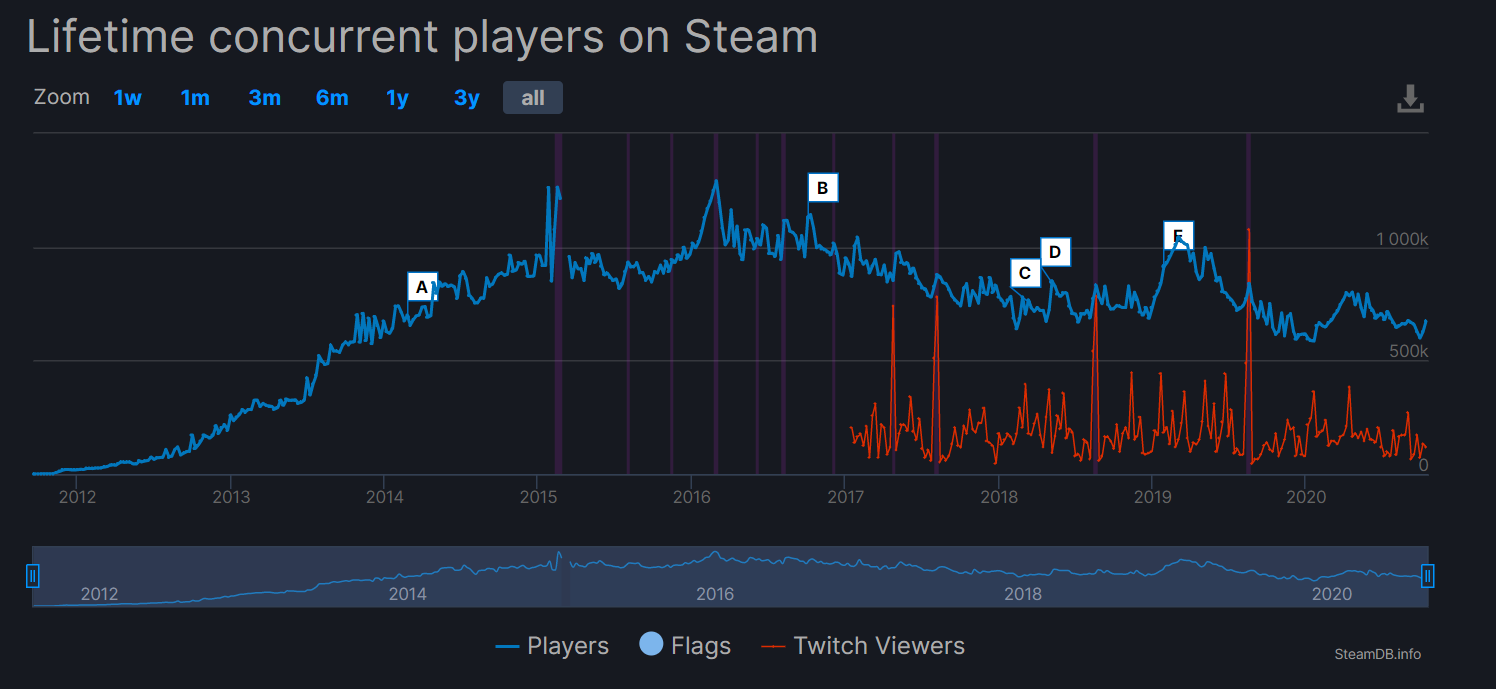
\includegraphics[scale = 0.5]{./img/steamDB.png}
    \centering
    \end{figure}

    \item Data Scraping \\
    Some scrappers deployed on GitHub were developed to scrape reviews data directly from the official website. Both the product information and user review information can be scraped. Most of the scrapers were built with python. The advantages of this methods is that these reviews are complete and updated. The disadvantage of this methods is that this time method is time consuming and sometimes when we hit the time limit, IP addresses might be banned by the sever adminstors.


    \item API \\ 
    The finally chosen method is the application programming interface. \\ 
    The reviews got from API are not in the real time manner but they are updated regualrly. Additionally, user infromation can be downloaded with user infromation API. But they are sometimes comes with a lot of missing values. 

\end{itemize}


\section*{Methodology}



    \subsection*{Data preprocess}
     I will use the $pre\_process\_text$ function (with different specifications such as stopwords, words stemming/lemmanization...etc) to convert the data into a sparse two-dimensional matrix, The rows represent the reviews and the columns represent each word within the reviews. Each element represents the number of appearance of each word in each review.


    
    \subsection*{Feature selection and vectorizer}
     After initial data preprocess, we use $N\_gram$ to generate feature. We will be trail with unigram, bigram and trigram. Since in some settings, we have negation words, bigram and trigram might perform better than unigram. For bigram, each pair of words ($word_1, word_2$) next to each other is selected as a feature. In represetation, a feature is associated with all the bigrams in the document. The feature value is defined as the number of appearances the bigram in the docuement. 
        
    \subsection*{TF/IDF}
     Term frequency and inverse docuemnt frequency. It is a vectorizer and transfromed data that can be used directly for the classification model. TFIDF can be used as a feature selection methods to select top $n$ features from all features with largest weight. The weights for each term is defined by taking average of that term in all docuemnts. The number of features selected for the final model can be chosen by cross validation. 
    

    \subsection*{Model\_1}
     The model used first will be \textbf{Gaussian Naive Bayes} (can obtained from $e107$ pacakge in R)  to train the model. The possible hyperparameters that can be tuned including N-gram, word window length, number of feartures, feature selection methods. upper and lower bound of the review text windw length. There are also additional features which is includes reviewer's playtime in the past 2 weeks, reviewer number of games owned, number of reviews reviewer made in the past. Cross validation is used for model selection. 75\% of all the data are randomly selected as the training data, and the remaining 25\% are test data.  

    \subsection*{Model\_2}
    The second model that I want  to predict sentiment will be from the sentimentR package in R. and I will trail with AFINN \& NRC dictionary to see which one has a better prediction (AUC score) \&\& $F_{beta}$ (Precision and recall) score. Potential hyperparameters that can be tuned: thresholds, word dictionaries, dtm text window length. 
    
    




\section*{Potential Challenges}

For the sentimentR pacakge, the challenge here no doubt is the computation time and the searching of optimal hyperparameters. From previous experiences, 10k observations normally takes an hour for the USF virtual machine to run. Each time if I want to tune the one of hyperparameters, the computational time increases exponentially.


For the Naive Bayes classifer model, the first challenge is the independence assumption, which is very hard to prove that with $top\_n$ features that we selected and the additional features we choose form the SteamDB are conditional independent. 

\begin{align*} 
  P(A|B) &=  \dfrac{P(AB)}{P(B)} \\ 
  P(AB) &=  P(B)P(A|B) \\ 
  P(AB) &= P(A) \times P(B|A) \\
  P(A) \times P(B|A) &= P(B)P(A|B) \\ 
  P(B|A) &= \dfrac{P(B)P(A|B)}{P(A)}
\end{align*}
Within the training dataset, if we assume each class $C$: 
$$C = (y_1, y_2...., y_{m})$$
and within each of the sample C, it has $n$ features and independent from each other, denoted as: 
$$ X = (x_1, x_2, x_3, ..., x_n)$$

under the conditional independence assumption, we can calculate the probability:
$$
\begin{aligned}
p\left(C_{k}, x_{1}, \ldots, x_{n}\right) &=p\left(x_{1}, \ldots, x_{n}, C_{k}\right) \\
&=p\left(x_{1} \mid x_{2}, \ldots, x_{n}, C_{k}\right) p\left(x_{2}, \ldots, x_{n}, C_{k}\right) \\
&=p\left(x_{1} \mid x_{2}, \ldots, x_{n}, C_{k}\right) p\left(x_{2} \mid x_{3}, \ldots, x_{n}, C_{k}\right) p\left(x_{3}, \ldots, x_{n}, C_{k}\right) \\
&=\cdots \\
&=p\left(x_{1} \mid x_{2}, \ldots, x_{n}, C_{k}\right) p\left(x_{2} \mid x_{3}, \ldots, x_{n}, C_{k}\right) \cdots p\left(x_{n-1} \mid x_{n}, C_{k}\right) p\left(x_{n} \mid C_{k}\right) p\left(C_{k}\right)
\end{aligned}
$$













\end{document}

